\section{Nominal Rigidity}


\subsection{Menu Costs}




    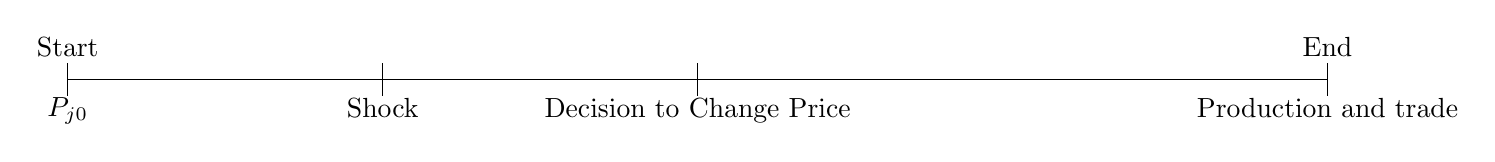
\begin{tikzpicture}[scale=2]
     % draw horizontal line   

      \draw (0,0) -- (8,0);



      % draw vertical lines
       \foreach \x in {0,2,4,8}
       \draw (\x cm,3pt) -- (\x cm,-3pt);

        % draw nodes
       \draw (0,0) node[below=3pt] {$P_{j0}$ } node[above=5pt] {Start};
       \draw (2,0) node[below=3pt] {Shock};
       \draw (4,0) node[below=3pt] {Decision to Change Price};
       \draw (8,0) node[below=3pt] {Production and trade} node[above=5pt] {End};

       \end{tikzpicture}
       
       
\paragraph{Partial Equilibrium analysis}
\begin{itemize}
    \item Monopolistic Competition
    \item Macroeconomic variables:
        \begin{itemize}
        \item $\overline{D}$ --- Demand is given
            \item $\mathbf{P} = \mathbf{\overline{P}}$ --- Prices are fixed and equal to the price index
            \item $n = \overline{n}$ --- The mass of contiuum of goods is fixed
        \end{itemize}
\end{itemize}

Demand for firm $j$ is given by:

$$
Y_j = Y_j\left(p_j ,D  \right) \implies p_j = p_j \left( Y_j, D  \right)
$$

Where 

\begin{align*}
    \frac{\partial Y}{\partial p_j} < 0 && \frac{\partial Y}{\partial D} > 0
\end{align*}

Meaning that the output for firm $j$ is decreasing in price and increasing in demand.

\paragraph{Choosing the initial price}

$$
\overline{D} = \overline{D}_0
$$

$$
w = \overline{w}_0
$$

$$
p_j \left( y_j, \overline{D}_0 \right) - \left( 1 - \frac{1}{\sigma_j}  \right) = MC(y_j) 
$$

2 Conditions for this period:
\begin{align*}
    \overline{D} = \overline{D} && w = \overline{w}
\end{align*}

Which means that the firm takes both the demand and wage as given. 

\paragraph{Changing the prices}

\begin{align*}
    p_{j1}^* = p_j \left( Y_{j1}^*, \overline{D}_1 \right) \\
    &&& p_{j1}^* =
\end{align*}

$$
TC_j = wf^{-'} \left(  \frac{y_j}{A_j}  \right)
$$

\subsubsection{Aggregate Demand Expansion}
$$\Delta \pi _ { j } = \pi_j - \pi^*_j = (D - A) + \Psi p$$

Price change iff:

$$\Delta \pi_j > 0 \implies \mathbf{P} \Psi > A - D$$

If the change in profit is positive, meaning that the menu cost is smaller than the gain in profit.


$$
\Delta CS = A + B > 0
$$

$$
\Delta SW = \Delta CS + \Delta \pi _ { j } = A + B + (D - A) + \Psi \implies
D + B + \mathbf{P} \Psi > 0
$$



\subsubsection{Aggregate Demand Contraction}

$$
\pi^*_{j1} - \pi_{j1} = (H - E) - \Psi \mathbf{P}
$$

A firm would keep their price unchanged iff:

$$
\Delta \pi < 0 \implies \mathbf{P} \Psi > H- E
$$

$$
\Delta CS  = E + F
$$

$$
\Delta SW = - \left(  \Delta CS + \Delta \pi_j  \right) \implies (E + F) + (H - E) - \Psi \mathbf{P} \implies F + H - \mathbf{P} \Psi
$$

From a social point of view it is preferable to keep prices unchanged iff the menu costs are larger than F + H, thus very large menu costs. Such large menu costs are not likely and we would not expect that the social optimum is to keep the prices unchanged. However, from the point of the view of the firm  

\subsubsection{General Equlibrum Model}

\paragraph{Assumptions}
\begin{enumerate}
    \item No Government: $G = T = 0$
    \item $M_E = \overline{M_E}$ --- Money endownment is fixed
    \item $A_j = 1$
    \item $B = 1$
    \item $\Phi = 0$ --- No fixed administrative costs
\end{enumerate}

Assumption 4 and 5 together tells us that we have Constant Returns to Scale in this case. 

\paragraph{Households}

$$
C = \gamma \alpha \frac { \overline { M _ { E } } + w + \pi } { \mathbf { P } }
$$

$$
M= ( 1 - \gamma) \left( \overline { M _ { E } } + w + \pi \right)
$$

$$
L = 1 - \gamma \left( 1 - \alpha  \right) \frac{\overline{M_E} + w + \pi}{w}
$$

Initial EQ:

$$
p_j \left(1 - \frac{1}{\sigma}  \right)  = w (MC)
$$

$$
\pi_j = p_j y_j - wN_j = \left( p_j - w  \right)y_j \implies \frac{p_j y_j}{\sigma}
$$

$$
\mathbf{P} = p_j
$$

$$
\pi = \frac{p y}{\sigma}
$$

$$
w = \mathbf{P} \frac{\sigma - 1}{\sigma}
$$

$$
C = ....
$$

$$
Y = C
$$

$$
Y = 1 \cdot N
$$

$$
N = L
$$

$$
L = ... insert
$$

$$
w = \mathbf{P} \frac{\sigma - 1}{\sigma}
$$

$$
\pi = \frac{p y}{\sigma}
$$

$$
M = ...
$$


\begin{align}
    Y = C \implies \\
    Y = \gamma \alpha \frac { \overline { M _ { E } } + w + \pi } { \mathbf { P } } \implies \\
    \overline{M_E} + w + \pi = \frac{p y}{\gamma \alpha}
\end{align}

\begin{align}
    Y = L \implies \\
    Y = L = 1 - \gamma \left( 1 - \alpha  \right) \frac{\overline{M_E} + w + \pi}{w} \implies \\
    Y_0^* = \frac{\alpha ( \sigma - 1 )}{\sigma - \alpha}
\end{align}


\begin{align}
    M_E + w + \pi = \frac{p y}{\gamma \alpha} \implies \\
    \mathbf{P_0^*} = \frac{\gamma (\sigma - \alpha}{(\sigma - 1)(1 - \gamma)}\overline{M_E}_0
\end{align}


Assumption:

$$
\overline{M_E}_0 = \frac{(\sigma - 1)(1 - \gamma)}{\gamma (\sigma - \alpha)} \implies \mathbf{P_0^*} = 1
$$

\paragraph{Monetary Shock with menu Costs}

$$
\mathbf{P} = \overline{\mathbf{P_0}} = 1
$$

$$
\pi = py - wN
$$


$$
Y = C ...
$$

\begin{align}
    Y = L \implies \\
    Y = 1 - \gamma \left( 1 - \alpha  \right) \frac{Y}{ \gamma \alpha w} \implies \\
    w = \frac{1 - \alpha}{\alpha} \cdot \frac{Y}{1 - Y}
\end{align}



$$
\pi = (1 - w)Y
$$

$$
\pi + w = ...... = \frac{Y}{\alpha}
$$


$$
Y = \gamma \alpha \left( \overline{M_E} + \frac{Y}{\alpha}     \right) \implies \\
Y = \frac{\gamma \alpha}{1 - \gamma}\overline{M_E} \implies \\
Y_1 = k \overline{M_E}
$$

Where $k$ is:

$$
k = \frac{\gamma \alpha}{1 - \gamma} > 0
$$


$$
 \left. \frac{\partial Y^*}{\partial \overline{M_E}} \right\rvert_{k} = \frac{\gamma}{(1 - \gamma)\mathbf{\overline{P_0^*}}}
 $$
 
 \paragraph{Welfare}
 
 $$
 U = \left[ C^{\alpha} (1-L)^{1-\alpha}   \right]^{\alpha} \cdot \left( \frac{M}{P}    \right)^{1 - \gamma}
 $$
 
 
 $$
 \Tilde{U} = \gamma \left[  \alpha \Tilde{C} + (1 - \alpha)\Tilde{Z}   \right] + (1 - \gamma)(\Tilde{M} - \mathbf{\Tilde{P}})
 $$

$$
L^* = Y^* \implies \Tilde{L} = \Tilde{Y}
$$

$$
Z = 1 - L \implies \Tilde{Z} = - \frac{dL}{1 - L_0^*} = \frac{Y_0^*}{1 - Y_0^*}\Tilde{Y}
$$


$$
\Tilde{U} = 
\left \{
\gamma \left[ \alpha - (1 - \alpha) \cdot \frac{\alpha (\sigma -1)}{\sigma (1 - \alpha)} + (1 - \gamma)  \right] M_E
\right \}
$$

In the above equation we have the following:
\begin{itemize}
    \item  The $\alpha$ co-responds to the change in consumption $\Delta C$
    \item Change in Liquidity Services + Real Money Balances
    \item Change in leisure, because output goes up people would have to work more which reduces Leisure. 
\end{itemize}

By simplifying you can arrive at:

$$
\Tilde{U} = \frac{\sigma (1 - \gamma)+\alpha \gamma}{\sigma} \overline{M_E}
$$

Welfare multiplier $V > 0$ Why?


$$
\mu_{Actual} = \frac{\mathbf{P} - w}{\mathbf{P}} = 1 - w \implies
1 - \frac {1 - \alpha } { \alpha } \cdot \frac { Y } { 1 - y }
$$

$$
d\mu_{Actual} = - \frac{1- \alpha}{\alpha} \cdot \frac{dY}{(1 - Y_0^*)^2}
$$

\paragraph{Notes on alternative 2 in GE}

$$
Y_j = \left( \frac{P_j}{\mathbf{P}}  \right)^{- \sigma} \left( \frac{C}{n} + \Psi   \right)
$$

$$
VA_j = \frac{p_j}{\mathbf{P}}Y_j - n\Psi \implies \sum_{j} VA_j = nY_j  - n \Psi
$$


$$
Y_1^* = 1 N - n \psi 
$$




$$
\pi_j^* = \mathbf{P}(Y + n \Psi) - wN - n\mathbf{P}\Psi = \mathbf{P}Y - w\Tilde{N}
$$



\subsubsection{Primary conclusions of the Menu Costs}
\begin{enumerate}[i]
  \item The existence of menu costs can lead to much larger losses in welfare, than the cost to the individual firm.
  \item Asymmetric incentives for firms: Adjustment is better with demand expansion, but worse with demand contractions.
  \item Menu costs are a short run market friction, in the long-run price will adjust to its natural level.
\end{enumerate}


\newpage
\subsection*{Time Dependent Models}
\subsection{A Particular Case: Calvo Pricing}

Exogenous decision on price changes, done by a random lottery. The lottery defines who can change prices, and who can't, not necessarily the actual changes in prices that ensue.  


\paragraph{}

\begin{figure}[ht]

\centering
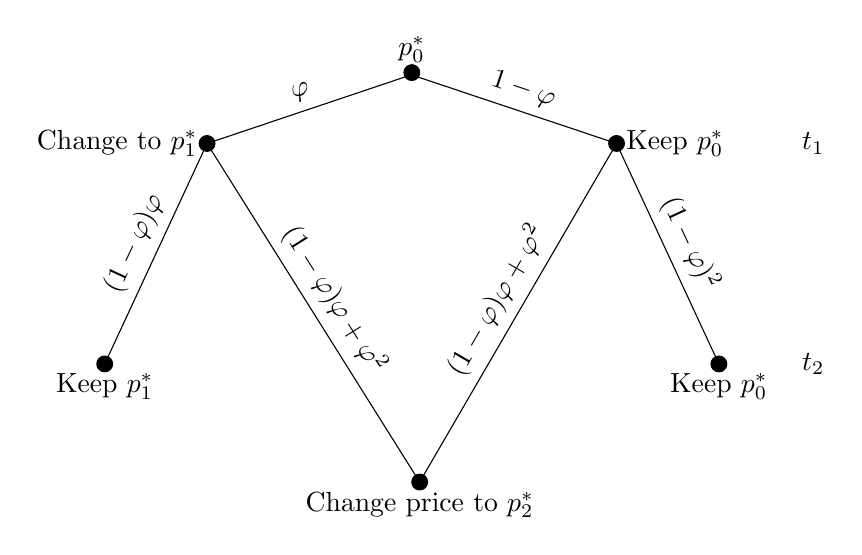
\begin{tikzpicture}[scale=1]


\coordinate (a) at (3.83, 2.65);
\coordinate (c) at (1.3, 1.8);
\coordinate (d) at (4, -2.5);
\coordinate (e) at (0,-1);
\coordinate (f) at (7.8, -1);




\draw [fill] (c) circle [radius=0.1] node [left] {Change to $p_1^*$};
\draw [fill] (6.5, 1.8) circle [radius=0.1] node [right] {Keep $p_0^*$};
\draw [fill = black] (3.9, 2.7) circle [radius=0.1] node [above] {$p_0^*$};
\draw [fill] (d) circle [radius=0.1] node [below] {Change price to $p_2^*$};
\draw [fill] (e) circle [radius=0.1] node [below] {Keep $p_1^*$};
\draw [fill] (f) circle [radius=0.1] node [below] {Keep $p_0^*$};


\draw (e)-- (c) node[pos=0.5,sloped,above] {$(1-\varphi)\varphi$};
\draw (a) -- (c) node[pos=0.5,sloped,above] {$\varphi$}; 




\draw (3.96, 2.65) -- (6.5, 1.8) node[pos=0.5,sloped,above] {$1-\varphi$};
\draw (6.5, 1.8) -- (7.8, -1) node[pos=0.5,sloped,above] {$(1-\varphi)^2$};
\node at  (9, 1.8) {$t_1$};
\node at  (9, -1) {$t_2$};


\draw (c) -- (d) node[pos=0.5,sloped,above] {$(1-\varphi)\varphi+\varphi^2$};
\draw (6.5, 1.8) -- (d) node[pos=0.5,sloped,above] {$(1-\varphi)\varphi+\varphi^2$};


\end{tikzpicture}
\caption{Decision tree}
\end{figure}

In the first period each firm has a probability $\varphi$ do be able to change prices, and a probability $(1- \varphi)$ that they can't.
In the second period: 
\begin{itemize}
    \item there is a probability $(1-\varphi)^2$ that companies that didn't change prices in the last period can't change prices again;
    \item a probability $(1-\varphi)\varphi$ that companies who changed prices last period can't change prices in this one;
    \item a probability $(1-\varphi)\varphi+\varphi^2$ that companies who either kept the last prices, or changed it in the last period, can change prices in this period;
\end{itemize}

And it goes like this for every period, until the last one where: 
\begin{itemize}
    \item $(1-\varphi)^{\tau}$ companies will have kept the first price $p^{*}_{0}$;
    \item $(1-\varphi)^{\tau -1}\varphi$ will have kept $p^{*}_{1}$;
    \item $(1-\varphi)^{\tau - 2}\varphi^2$ will have kept $p^{*}_{2}$;
    \item And so on.
\end{itemize}

If $\varphi =1$, companies can always choose to change prices, and the condition for their price comes as: 
\begin{equation*}
    p^{*}_{j\tau}.(1+\frac{1}{\varepsilon_{j\tau}})=MC_{j\tau}
\end{equation*}
This means that companies will always be changing prices to adjust to their marginal cost, and the elasticities they face, if they need to. 

\paragraph{}
\subsubsection{Micro Foundations}
The problem of the firm comes, in this situation, as: 

\begin{equation*}
    \underset{p_{j\tau}}{max} E_{t}\sum_{\tau=t}^{\infty}(1+\rho)^{-(\tau-t)}.(1-\varphi)^{\tau-t}.\pi(p_{j\tau})
\end{equation*}

Where 
\begin{equation*}
\begin{aligned}
\pi(p_{j\tau})=p_{j\tau}.y_{j\tau}-w_{\tau}.N_{j\tau} \\
\pi(p_{j\tau})=p_{j\tau}(\frac{p_{j\tau}}{P})^{-\sigma}D_{t}-w_{\tau}\frac{y_{j\tau}}{A_{\tau}} \\
\pi(p_{j\tau})=P_{\tau}^{\sigma}D_{\tau}-(p_{j\tau}^{1-\sigma}.\frac{w_{\tau}}{A_{\tau}}.p_{j\tau}^{-\sigma})
\end{aligned}
\end{equation*}
Note that $y_{j\tau}$ is the same as $y_{j}$ in the last section. Also $\frac{w_{\tau}}{A_{\tau}}$ is the Marginal Cost at period $\tau$.

Substituting in the maximization problem, comes:

\begin{equation}
     \underset{p_{j\tau}}{max} \sum_{\tau=t}^{\infty}(\frac{1-\varphi}{1+\rho})^{\tau-t}E_{t}[P_{\tau}^{\sigma}D_{\tau}-(p_{j\tau}^{1-\sigma}.\frac{w_{\tau}}{A_{\tau}}.p_{j\tau}^{-\sigma})]
\end{equation}

Let's call the equation being maximized, $V_{t}$.

\begin{equation*}
    \frac{\partial V_{t}}{\partial p_{j\tau}}=0 \\
    \implies \sum_{\tau=t}^{\infty}(\frac{1-\varphi}{1+\rho})^{\tau-t}.E_{t}\frac{\partial \pi_{j\tau}}{\partial p_{j\tau}}=0
\end{equation*}

\begin{equation*}
\begin{aligned}
    E_{t}\frac{\partial \pi_{j\tau}}{\partial p_{j\tau}}=E_{t}[(1-\sigma)P_{\tau}^{\sigma}D_{\tau}p_{j\tau}^{-\sigma}+\sigma\frac{w_{\tau}}{P_{\tau}}P_{\tau}D_{\tau}p_{j\tau}^{-(-\sigma-1)}] \\
    E_{t}\frac{\partial \pi_{j\tau}}{\partial p_{j\tau}}=(\sigma-1)E_{t}[P_{\tau}D_{\tau}.p_{j\tau}^{-(\sigma-1)}(p_{j\tau}^{*}-p_{j\tau}] \\
    \text{Where,} && p_{j\tau}^{*}=\frac{\sigma}{\sigma-1}\frac{w_{\tau}}{A_{\tau}}
\end{aligned}
\end{equation*}

In the Steady State: 
\begin{equation*}
    p_{j\tau}^{*}=p^{*} \implies y_{j\tau}^{*}=(\frac{p^{*}}{P^{*}})^{-\sigma}.\frac{D^{*}}{n=1} \implies y_{j\tau}^{*}=D^{*}
\end{equation*}
    
\begin{equation*}
\begin{aligned}
    dE_{t}X_{\tau}(p_{j\tau}^{*}-p_{j\tau})=E_{t}(p^{*}-p^{*})dX_{\tau}+X^{*}(dp_{j\tau}^{*}-dp_{j\tau}) \\
    \text{Where,} && X_{\tau}=P_{\tau}^{\sigma}D_{\tau}p_{j\tau}^{-\sigma-1} \\
    E_{t}[P^{*\sigma}D^{*}p^{*(-\sigma-1)}(dp_{j\tau}^{*}-dp_{j\tau})]E_{t}[D^{*}(\Tilde{p_{j\tau}^{*}}-\Tilde{p}_{j\tau})]=D^{*}E_{t}[\Tilde{p}_{j\tau}^{*}-p_{j\tau}]
\end{aligned}
\end{equation*}

From here we take the optimal pricing rule in the Calvo Model:

\begin{equation}
    \sum^{\infty}_{\tau=t}(\frac{1-\varphi}{1+\rho})^{\tau-t}E_{t}(\Tilde{p_{j\tau}^{*}}-\Tilde{p_{j\tau}})\simeq 0 
\end{equation}

Note that $p_{j\tau}=p_{j\tau}^{*}(1+\Tilde{p}_{j\tau})$

\begin{equation*}
   \begin{aligned}
    \sum^{\infty}_{\tau=t}(\frac{1-\varphi}{1+\rho})^{\tau-t}\Tilde{p}_{j\tau}=\sum^{\infty}_{\tau=t}(\frac{1-\varphi}{1+\rho})^{\tau-t}E_{t}p_{j\tau}^{*} \\ \text{Where,} && \Tilde{p}_{j\tau}=\Tilde{p}_{jt} \\
    \Tilde{p}_{jt}\sum^{\infty}_{\tau=t}(\frac{1-\varphi}{1+\rho})^{\tau-t}=\Tilde{p}_{jt}\frac{1}{1-\frac{1-\varphi}{1+\rho}} \\
    \Tilde{p}_{jt}\frac{\varphi+\rho}{1+\rho}=\sum^{\infty}_{\tau=t}(\frac{1-\varphi}{1+\rho})^{\tau-t}E_{t}p_{jt}^{*} \\ 
   \implies \Tilde{p}_{jt}=\sum^{\infty}_{\tau=t}\varpi_{\tau-t}E_{t}\Tilde{p}_{j\tau}^{*}
   \end{aligned}
\end{equation*}
$\varpi_{\tau-t}$ comes as:
\begin{equation*}
       \varpi_{\tau-t}=\frac{\varphi+\rho}{1+\rho}(\frac{1-\varphi}{1+\rho})^{\tau-t} 
\end{equation*}

And follows the condition:
\begin{equation*}
        \sum^{\infty}_{\tau=t}\varpi_{\tau-t}=1
\end{equation*}

To finish defining the micro variables in the model: 
\begin{equation*}
    \begin{aligned}
        p_{j\tau}=\frac{\sigma}{\sigma-1}.MgC_{j\tau} \\
        \Tilde{p}_{j\tau}=\Tilde{MgC}_{j\tau} \\
        \Tilde{MgC}_{j\tau}=\rho_{MgC}\Tilde{MgC}_{j,\tau-1}+\varepsilon_{MgC,\tau}
    \end{aligned}
\end{equation*}
Note the Marginal Cost is determined by an AR(1) process.

\subsubsection{Aggregate Dynamics}
Assume a fixed number of companies $n_{t}=\overline{n}$.
In the Steady State, $p_{j\tau}=p^{*}$, and $P_{t}^{*}=p_{t}^{*}$.

\begin{equation*}
    P_{t}=(\frac{1}{n}\sum^{\overline{n}}_{j=1}p_{jt}^{1-\sigma})^{\frac{1}{1-\sigma}}
\end{equation*}

\begin{equation*}
      dP_{t}=\frac{1}{1-\sigma}(\frac{1}{n}\sum^{\overline{n}}_{j=1}p^{*(1-\sigma)})^{\frac{1}{1-\sigma}-1}(1-\sigma)\frac{1}{n}\sum^{\overline{n}}_{j=1}p^{*-\sigma}dp_{jt} 
\end{equation*}

\begin{equation*}
\begin{aligned}
    dP_{t}=\frac{1}{\overline{n}}\sum^{\overline{n}}_{j=1}dp_{jt} \\
    \Tilde{P}_{t}=\frac{1}{\overline{n}}\sum^{\overline{n}}_{j=1}\Tilde{p}_{jt}
\end{aligned}
\end{equation*}

The number of companies that set a price different from that of the last period is given by $\varphi.\overline{n}$. With the old prices there are $(1-\varphi)\overline{n}$.

\paragraph{}
Let's see the aggregate price levels in different periods. Starting with $t=1$:

\begin{equation*}
    \Tilde{P}_{1}=\frac{1}{\overline{n}}[\varphi.\overline{n}+(1+\varphi)\overline{n}.\Tilde{p}_{0}]=\varphi\Tilde{p}_{1}+(1+\varphi)\Tilde{p}_{o}=\varphi\Tilde{p}_{1}
\end{equation*}
Because $\Tilde{p}_{0}=0$.
For $t=2$:
\begin{equation*}
    \Tilde{P}_{2}=\frac{1}{\overline{n}}[\varphi\overline{n}.\Tilde{p}_{1}+(1-\varphi)\overline{n}.\Tilde{p}_{0}]=\varphi\Tilde{p}_{2}+(1+\varphi)\Tilde{P}_{1}
\end{equation*}
By the same rationale, we can generalize for any period t, 
\begin{equation} \label{Price_aggregate_Calvo}
\begin{aligned}
    \Tilde{P}_{t}=\varphi\Tilde{p}_{t}+(1-\varphi)\Tilde{P}_{t-1} \\
    \Tilde{P}_{t}=\varphi\sum^{\infty}_{\tau=t}\varpi_{\tau-t}E_{t}\Tilde{P}_{t}^{*}+(1+\varphi)\Tilde{P}_{t-1}
\end{aligned}
\end{equation}

We can now look at the evolution of inflation $\pi_{t}$

\begin{equation*}
    \pi_{t}=\frac{P_{t}}{P_{t-1}}-1 \implies 1+\pi_{t}=\frac{P_{t}}{P_{t-1}}
\end{equation*}

Translating this to the notation on our model, 
\begin{equation*}
    \pi_{t}=\Tilde{P}_{t}-\Tilde{P}_{t-1}=\varphi\big(\sum^{\infty}_{\tau=t}\varpi_{\tau-t}E_{t}P_{\tau}^{*}-\Tilde{P}_{t-1}\big)
\end{equation*}

\subsubsection{Inflation in a simple New Keynesian Model}
\begin{equation}
\begin{aligned}
    \Tilde{p}_{t}=\frac{\varphi+\rho}{1+\rho}\sum^{\infty}_{\tau=t}\big(\frac{1-\varphi}{1+\rho}\big)^{\tau-t}E_{t}\Tilde{p}_{\tau}*{*} \\
    \Tilde{p}_{t}=\frac{\varphi+\rho}{1+\rho}\Tilde{p}_{t}^{*}+\frac{\varphi+\rho}{1+\rho}\sum^{\infty}_{\tau=t+1}\big(\frac{1-\varphi}{1+\rho}\big)^{\tau-t}\Tilde{p}_{t}^{*} \\ 
     \Tilde{p}_{t}=\frac{\varphi+\rho}{1+\rho}\Tilde{p}_{t}^{*}+\frac{1-\varphi}{1+\rho}\frac{\varphi+\rho}{1+\rho}\sum^{\infty}_{\tau=t}\bigg (\frac{1-\varphi}{1+\rho} \bigg)^{\tau-t}E_{t}\Tilde{p}_{t+1} \\
     \Tilde{p}_{t}=\frac{\varphi+\rho}{1+\rho}\Tilde{p}_{t}+\frac{1-\varphi}{1+\rho}E_{t}\Tilde{p}_{t+1} \\
    \Tilde{p}_{t}=(1-\xi)\Tilde{p}_{t}^{*}+\xi E_{t}\Tilde{p}_{t+1}
\end{aligned}
\end{equation}

Where, 
\begin{equation*}
    \xi=\frac{1-\varphi}{1+\rho}
\end{equation*}

Recalling the first equation in \ref{Price_aggregate_Calvo}, we can get a function for the aggregate price change in $t+1$, as: 

\begin{equation*}
\begin{aligned}
E_{t}\Tilde{P}_{t+1}=\varphi E_{t}\Tilde{p}_{t+1}+(1-\varphi)\Tilde{P}_{t} \\
E_{t}\Tilde{p}_{t+1}=\frac{1}{\varphi}\bigg[E_{t}\Tilde{P}_{t+1}-(1-\varphi)\Tilde{P}_{t}\bigg] \\ 
\Tilde{p}_{t}=(1+\xi)\Tilde{P}_{t}+\xi\frac{1}{\varphi}\bigg[E_{t}\Tilde{P}_{t+1}-\Tilde{P}_{t}+\varphi\Tilde{P}_{t}\bigg] \\ 
\Tilde{p}_{t}=(1+\xi)\Tilde{P}_{t} +\xi\Tilde{P}_{t}+\frac{\xi}{\varphi}E_{t}\pi_{t+1}
\end{aligned}
\end{equation*}

\begin{equation*}
\begin{aligned}
    \pi_{t}=\varphi(\Tilde{P}_{t}-\Tilde{P}_{t-1}) \\ 
\end{aligned}
\end{equation*}

\begin{equation} \label{New_Keynesian_Phillips}
    \pi_{t}= K(\Tilde{P}_{t}^{*}-\Tilde{P}_{t-1})+\beta E_{t}\pi_{t+1}
\end{equation}

Where, $ K=\frac{\varphi(1-\xi)}{1-\xi \rho} > 0$, and $\beta = \frac{\xi}{1-\varphi \xi} > 0$.

\paragraph{}
Note that $(\Tilde{P}_{t}^{*}-\Tilde{P}_{t-1})$ in \ref{New_Keynesian_Phillips} is a sort of output gap. To make it more clear, recall: 

\begin{equation*}
    P_{t}^{*}=(1-\frac{1}{\sigma}).\frac{w_{t}}{A_{t}} \implies\Tilde{P}_{t}^{*}=\Tilde{w}_{t}-\Tilde{A}_{t}
\end{equation*}

And from the real business cycle model: 
\begin{equation*}
    \Tilde{L}_{t}=\frac{1-L^{*}}{L_{*}}\bigg(\frac{1}{\chi}\Tilde{w}_{t}-\frac{\theta}{\chi}\Tilde{c}_{t}\bigg) \implies \Tilde{w}_{t}-\theta\Tilde{L}_{t}=\frac{\chi-L^{*}}{1-L^{*}}
\end{equation*}

Using a simple production function that uses only labour, 

\begin{equation*}
    Y_{t}=A_{t}N_{t} \implies \Tilde{N}_{t}=\Tilde{L}_{t}=\Tilde{Y}_{t}-\Tilde{A}_{t}
\end{equation*}
In this model there is only consumption, so $Y_{t}=c_{t} \implies \Tilde{c}_{t}=\Tilde{Y}_{t}$

\begin{equation*}
    \Tilde{w}_{t}=\frac{\chi.L^{*}}{1-L^{*}}(\Tilde{Y}_{t}-\Tilde{A}_{t})+\theta\Tilde{Y}_{t}
\end{equation*}

With all this we get a new, more specified equation for the \textbf{New Keynesian Phillips Curve}, 

\begin{equation}
    \pi_{t}=K\bigg[\big(\frac{\chi.L^{*}}{1-L^{*}}+\theta \big)\Tilde{Y}_{t}-\big(1+\frac{\chi.L^{*}}{1-L^{*}} \big)\Tilde{A}_{t}-\Tilde{P}_{t+1}\bigg]
\end{equation}

Look now at the implications of the values on $\varphi$. If firms are completely free to change their prices, $\varphi=1 \implies \xi=0 \implies K=1$ and $\beta=0$. 
\paragraph{}
If firms can never change their prices, then $\varphi=0 \implies \xi=\frac{1}{1+\rho} \implies K=0$ and $\beta=\xi=\frac{1}{1+\rho}$



\begin{tcolorbox}
\subsection*{Calvo and Menu Costs Link}
\tcblower
Firms that are not able to change their prices, can be seen as firms who have an infinitely large menu cost. Because they are not winning the price-changing lottery they will be stuck with their old price and not being able to react to demand shocks. 
\end{tcolorbox}